\documentclass[paper=a4,twoside=false,fontsize=11pt,numbers=noenddot,version=first,bibliography=totoc,headsepline]{scrbook}

% Get the necessary packages for the document.
\input{Packages}
% Get the new commands we defined for this document.
% The name of Kieker, just for the case that the design of this should change.
\newcommand{\Kieker}{\textsf{Kieker}}

% The current version-string.
\newcommand{\version}{1.14} % will be set automatically by ant 'release' target 

% The single parts of Kieker and some files.
\newcommand{\KiekerMonitoringPart}{\textsf{Kieker.\-Monitoring}}
\newcommand{\KiekerAnalysisPart}{\textsf{Kieker.\-Analysis}}
\newcommand{\KiekerTraceAnalysis}{\textsf{Kieker.Trace\-Analysis}}
% \newcommand{\analysisJar}{kieker-analysis-\version.jar}
\newcommand{\mainJar}{kieker-1.14.jar} % will be set automatically by ant 'release' target
\newcommand{\mainJarEMF}{kieker-1.14-emf.jar} % will be set automatically by ant 'release' target
\newcommand{\mainJarWeaver}{kieker-1.14-aspectj.jar} % will be set automatically by ant 'release' target
% \newcommand{\monitoringJar}{kieker-monitoring-\version.jar}
% \newcommand{\commonJar}{kieker-common-\version.jar}
% \newcommand{\toolsJar}{kieker-tools-\version.jar}
\newcommand{\commonsLoggingJar}{commons-logging-1.1.2.jar}
\newcommand{\aspectJWeaverJar}{aspectjweaver-1.8.2.jar}
\newcommand{\monitoringPropertiesFile}{kieker.\-monitoring.\-pro\-per\-ties}
\newcommand{\analysisPropertiesFile}{kieker.analysis.properties}
\newcommand{\sigarJar}{sigar-1.6.4.jar}

\newcommand{\aopConfigFile}{aop.xml}
\newcommand{\binaryFileForDownload}{kieker-\version{}\-bina\-ries.zip}
\newcommand{\kiekerMonitoringProperties}{kieker.monitoring.pro\-perties}
\newcommand{\kiekerExampleMonitoringProperties}{kieker.monitoring.ex\-am\-ple.pro\-perties}

%%
\newcommand{\aspectJURL}{www.eclipse.org/aspectj/}

% Some directories for the examples
\newcommand{\userGuideDir}{kieker-documentation/userguide}
\newcommand{\exampleDir}{kieker-examples/userguide}
\newcommand{\exampleDirWin}{kieker-examples\textbackslash{}userguide}
\newcommand{\exampleDirRelativePath}{../../\exampleDir}
\newcommand{\plainBookstoreApplicationDir}{\exampleDirRelativePath/ch2--bookstore-application}
\newcommand{\plainBookstoreApplicationDirDistro}{\exampleDir/ch2--bookstore-application}
\newcommand{\manualInstrumentedBookstoreApplicationDir}{\exampleDirRelativePath/ch2--manual-instrumentation}
\newcommand{\manualInstrumentedBookstoreApplicationDirDistro}{\exampleDir/ch2--manual-instrumentation}
\newcommand{\customComponentsBookstoreApplicationDir}{\exampleDirRelativePath/ch3-4--custom-components}
\newcommand{\customComponentsBookstoreApplicationDirDistro}{\exampleDir/ch3-4--custom-components}
\newcommand{\aspectJBookstoreApplicationDir}{\exampleDirRelativePath/ch5--trace-monitoring-aspectj}
\newcommand{\aspectJBookstoreApplicationDirDistro}{\exampleDir/ch5--trace-monitoring-aspectj}
\newcommand{\aspectJBookstoreApplicationDirDistroWin}{\exampleDirWin\textbackslash{}ch5--trace-monitoring-aspectj}

\newcommand{\exampleReleaseDir}{examples/userguide}
\newcommand{\exampleReleaseDirWin}{examples\textbackslash{}userguide}
\newcommand{\exampleReleaseDirRelativePath}{../../\exampleReleaseDir}
\newcommand{\plainBookstoreApplicationReleaseDir}{\exampleReleaseDirRelativePath/ch2--bookstore-application}
\newcommand{\plainBookstoreApplicationReleaseDirDistro}{\exampleReleaseDir/ch2--bookstore-application}
\newcommand{\manualInstrumentedBookstoreApplicationReleaseDir}{\exampleReleaseDirRelativePath/ch2--manual-instrumentation}
\newcommand{\manualInstrumentedBookstoreApplicationReleaseDirDistro}{\exampleReleaseDir/ch2--manual-instrumentation}
\newcommand{\customComponentsBookstoreApplicationReleaseDir}{\exampleReleaseDirRelativePath/ch3-4--custom-components}
\newcommand{\customComponentsBookstoreApplicationReleaseDirDistro}{\exampleReleaseDir/ch3-4--custom-components}
\newcommand{\aspectJBookstoreApplicationReleaseDir}{\exampleReleaseDirRelativePath/ch5--trace-monitoring-aspectj}
\newcommand{\aspectJBookstoreApplicationReleaseDirDistro}{\exampleReleaseDir/ch5--trace-monitoring-aspectj}
\newcommand{\aspectJBookstoreApplicationReleaseDirDistroWin}{\exampleReleaseDirWin\textbackslash{}ch5--trace-monitoring-aspectj}



\newcommand{\kiekerSrcDir}{../../src/}

\newcommand{\distributedTestdataDir}{\aspectJBookstoreApplicationDir/testdata/kieker-20100830-082225522-UTC}
\newcommand{\distributedTestdataDirDistro}{\aspectJBookstoreApplicationDirDistro/testdata/kieker-20100830-082225522-UTC}
\newcommand{\distributedTestdataDirDistroWin}{..\textbackslash{}\aspectJBookstoreApplicationDirDistroWin\textbackslash{}testdata\textbackslash{}kieker-20100830-082225522-UTC}

\newcommand{\distributedTestdataReleaseDir}{\aspectJBookstoreApplicationReleaseDir/testdata/kieker-20100830-082225522-UTC}
\newcommand{\distributedTestdataReleaseDirDistro}{\aspectJBookstoreApplicationReleaseDirDistro/testdata/kieker-20100830-082225522-UTC}
\newcommand{\distributedTestdataReleaseDirDistroWin}{..\textbackslash{}\aspectJBookstoreApplicationReleaseDirDistroWin\textbackslash{}testdata\textbackslash{}kieker-20100830-082225522-UTC}

\newcommand{\JMSBookstoreApplicationDir}{\exampleDirRelativePath/appendix-JMS}
\newcommand{\JMSBookstoreApplicationReleaseDir}{\exampleReleaseDirRelativePath/appendix-JMS}
\newcommand{\JMSBookstoreApplicationDirDistro}{\exampleDir/appendix-JMS}
\newcommand{\JMSBookstoreApplicationReleaseDirDistro}{\exampleReleaseDir/appendix-JMS}

\newcommand{\AMQPBookstoreApplicationDir}{\exampleDirRelativePath/appendix-AMQP}
\newcommand{\AMQPBookstoreApplicationReleaseDirDistro}{\exampleReleaseDir/appendix-AMQP}

\newcommand{\SigarExampleDir}{\exampleDirRelativePath/appendix-Sigar}
\newcommand{\SigarExampleDirDistro}{\exampleDir/appendix-Sigar}
\newcommand{\SigarExampleReleaseDirDistro}{\exampleReleaseDir/appendix-Sigar}

\newcommand{\JavaEEServletExampleName}{JavaEEServletContainerExample}
\newcommand{\JavaEEServletExampleDir}{../../kieker-examples/\JavaEEServletExampleName}
\newcommand{\JavaEEServletExampleDirDistro}{kieker-examples/\JavaEEServletExampleName}
\newcommand{\JavaEEServletExampleReleaseDir}{../../examples/\JavaEEServletExampleName}
\newcommand{\JavaEEServletExampleReleaseDirDistro}{examples/\JavaEEServletExampleName}

% The complete url where to find Kieker.
\newcommand{\KiekerURL}{\url{http://kieker-monitoring.net}} 
% \newcommand{\KiekerDownloadURL}{\url{http://sourceforge.net/projects/kieker/files}}
\newcommand{\KiekerDownloadURL}{\url{http://kieker-monitoring.net/download/}}

% This is how we call the kieker directory.
\newcommand{\KiekerDir}{kieker-\version{}}%{$<$KIEKER-DIR$>$}

% These commands are necessary to mark classes, methods and files within the document.
\newcommand{\object}[1]{\texttt{#1}}
\newcommand{\class}[1]{\texttt{#1}}
\newcommand{\method}[1]{\textit{#1}}
\newcommand{\dir}[1]{\texttt{#1}}
\newcommand{\file}[1]{\texttt{#1}}
\newcommand{\parameterValue}[1]{\texttt{#1}}
\newcommand{\hostname}[1]{\texttt{#1}}

% This command formats the "new" files within a directory tree to get the users attention.
\newcommand{\newFilesDirTreeFormat}{\color{blue}}
\newcommand{\DirInDirTree}[1]{\textbf{#1}}
\newcommand{\newFileDirInDirTree}[1]{\colorbox{gray}{\color{white}#1}}


% These commands are for notifying the reader about something important.
\newcommand{\marginbox}[1]{\todo[noline]{#1}}
\newcommand{\notify}{\marginbox{\huge{\rightpointleft}}}
\newcommand{\warning}{\marginbox{\huge{\Stopsign}}}

% TODO command for our document
\newcommand{\TODO}[1]{\todo[inline,color=green!40]{TODO: #1}}

\makeatletter
\newcommand{\SYMBOLBOX}[2]{%
\begin{lrbox}{\@tempboxa}
\begin{minipage}[t]{0.1\textwidth}\vspace{1pt}
\begin{center}
\huge#1
\end{center}
\end{minipage}
\begin{minipage}[t]{0.8\textwidth}
#2%
\end{minipage}
\end{lrbox}
\todo[inline,bordercolor=black]{\usebox{\@tempboxa}}
}
\makeatother

\newcommand{\NOTIFYBOX}[1]{\SYMBOLBOX{\leftpointright}{#1}}
\newcommand{\WARNBOX}[1]{\SYMBOLBOX{\Stopsign}{#1}}

% This color will be used as backgroundcolor for the listings.
\definecolor{verylightgray}{gray}{.95}

% workaround for the listing's commentstyle
\newcommand{\textrmit}[1]{\textit{\textrm{#1}}}

% The following commands set the listings for the different (programming) languages correctly.
% For the first they use all nearly the same settings.
\newcommand{\setListing}[4]{
\lstset{    
numbers=#2,
basicstyle=#3,       	% the size of the fonts that are used for the code
keywordstyle=\bfseries,%
commentstyle={\textrmit},
showspaces=false,               % show spaces adding particular underscores
showstringspaces=false,         % underline spaces within strings
showtabs=false,                 % show tabs within strings adding particular underscores
%frame=shadowbox,	                % adds a frame around the code
% frame=lrtb,
rulesepcolor=\color{black},
linewidth=1\columnwidth,
columns=[c]flexible, % default is [c]fixed
% xleftmargin=1cm,
tabsize=2,	                % sets default tabsize to 2 spaces
captionpos=b,                   % sets the caption-position to bottom
breaklines=true,                % sets automatic line breaking
breakatwhitespace=false,        % sets if automatic breaks should only happen at whitespace
title=\lstname,                 % show the filename of files included with \lstinputlisting; also try caption instead of title
escapechar={#4},
backgroundcolor=\color{verylightgray},
style=#1, % they style may override one or more of the above settings
}
}

\lstdefinestyle{javaStyle}{
language=Java
}
\lstdefinestyle{bashStyle}{
language=Bash,
alsoletter={.,-,:}, % sonst auch 'java' in ClassName.java highlighted
morekeywords={java,javac,-classpath,-d,-jar,-javaagent:,copy,cp,dot,pic2plot,mkdir},
xleftmargin=3mm,
% showspaces=true
% emphstyle=\bfseries
}
\lstdefinestyle{xmlStyle}{
language=XML
}
\lstdefinestyle{PropertiesStyle}{
language=Bash,
xleftmargin=0mm
}
\lstdefinestyle{AntStyle}{
language=Ant,
xleftmargin=0mm
}
\lstdefinestyle{textStyle}{
language=,
xleftmargin=3mm
}

\newcommand{\UnixLikeSystem}{UNIX-like system}
\newcommand{\UnixLikeSystems}{UNIX-like systems}
\newcommand{\lstshellprompt}{$\triangleright$}
\newcommand{\lstHighlight}{\bfseries}
\newcommand{\setJavaCodeListing}{\setListing{eclipse-java}{left}{\sffamily\scriptsize}{\#}}
\newcommand{\setBashListing}{\setListing{bashStyle}{none}{\sffamily\footnotesize}{\#}}
\newcommand{\setPropertiesListing}{\setListing{PropertiesStyle}{none}{\sffamily\footnotesize}{}}
\newcommand{\setAntListing}{\setListing{AntStyle}{none}{\sffamily\footnotesize}{}}
\newcommand{\setTextListing}{\setListing{textStyle}{none}{\sffamily\scriptsize}{\$}}
\newcommand{\setXMLListing}{\setListing{xmlStyle}{left}{\sffamily\footnotesize}{}}

% This is the definition for the environment, that can be used for the background of the dirtrees.
\makeatletter\newenvironment{graybox}{%
   \begin{lrbox}{\@tempboxa}\begin{minipage}{0.965\columnwidth}}{\end{minipage}\end{lrbox}%
   \fcolorbox{white}{verylightgray}{\usebox{\@tempboxa}}
}\makeatother


\pagestyle{scrheadings}
\clearscrheadfoot

\ifoot[\hrule\sffamily Kieker \version{} User Guide]{\hrule\sffamily Kieker \version{} User Guide}
\ofoot[\hrule\sffamily\pagemark]{\hrule\sffamily\pagemark}

% Set the title and everything.
\titlehead{
  \begin{center}
    \includegraphics[height=25mm]{./images/20120511-kieker-logo-1-6}\\
\href{http://kieker-monitoring.net}{\sffamily\Large http://kieker-monitoring.net}
  \end{center}
}

\title{%
\Huge\Kieker{} \version{} User Guide%
\footnote{\sffamily \textit{For guidelines on how to cite Kieker and this document, please see~Section~\ref{sec:ch1:citingKieker}.}}
}

\author{\sffamily Kieker Project%
% , and contributors
}
\date{\sffamily\today}
% \date{\sffamily May 19, 2011}
\publishers{\normalsize\sffamily

\begin{center}
\begin{tabular}{cc}
Kiel University & University of Stuttgart\\
Department of Computer Science & Institute of Software Technology\\
Software Engineering Group & Reliable Software Systems Group \\
Christian-Albrechts-Platz 4 & Universitätsstra\ss{}e 38\\
24118 Kiel, Germany & 70569 Stuttgart, Germany
\end{tabular}
\end{center}


%\flushleft
% \includegraphics[height=2.5cm]{./images/caulogo}\\[0.5ex]

}

\hypersetup
{%
pdftitle = {\Kieker{} \version{} User Guide},
pdfauthor = {Nils Ehmke, Andr\'e van Hoorn, and Reiner Jung}
% colorlinks = {true}
}

% Here we go.
\begin{document}
  % We want a table of contents separated from the rest of the text.
  \maketitle
  \setcounter{tocdepth}{1} % not deeper than section level
  {\sffamily\tableofcontents}

  % Insert the other parts of the document.
  %%%%%%%%%%%%%%%%%%%%%%%%%%%%%%%%%%%%%%%%%
% Introduction
%
% $Date$
% $Revision$
% $Author$


\chapter{Introduction}\label{chap:introduction}

Modern software applications are often complex and have to fulfill a large set of functional and non-functional requirements. The internal behavior of such large systems cannot easily be determined on the basis of the source code. Furthermore, existing applications often lack sufficient documentation which makes it cumbersome to extend and change them for future needs. A solution to these problems can be dynamic analysis based on application-level monitoring, which allows to log the behavior of the application and to discover, for example, application-internal control flows, calling dependencies, and method response times.

Dynamic analysis can help in detecting performance problems and faulty behavior, capacity planning, and many other areas. The \Kieker{} framework provides the necessary monitoring capabilities and comes with tools and libraries for the analysis of monitored data. \Kieker{} has been designed for %
continuous monitoring in production systems inducing only a very low overhead. Further information on the overhead caused by \Kieker{} is provided at \url{http://kieker-monitoring.net/overhead-evaluation/}.
%, and offline evaluation of monitored data for a deeper inspection of the application's behavior and runtime architecture.

Please note that this document is aging.
We have started to transfer its content to our wiki \url{https://kieker-monitoring.atlassian.net/wiki/discover/all-updates}.

%%
\section{What is \Kieker?}\label{sec:kieker}



\Kieker{} is a Java-based application performance monitoring and dynamic software analysis framework~\cite{KiekerICPE2012}. %
Monitoring adapters for other platforms, such as Visual Basic~6~(VB6), .NET, and COBOL, exist as well.%
\footnote{\href{http://kieker-monitoring.net/support/}{Contact us} directly if you are interested in \Kieker{} support for other platforms} %
Figure \ref{fig:KiekerComponentDiagram} shows the framework's composition based %
on the two main components \KiekerMonitoringPart{} and \KiekerAnalysisPart{}. %

% This is the component diagram of Kieker (the satellite).
\begin{figure}[H]\centering
\includegraphics[width=0.96\textwidth]{images/kiekerComponentDiagram-woCloud-bw-w-record-newNames-withTraceAnalysis-colors}
\caption{Overview of the framework components}
\label{fig:KiekerComponentDiagram}
\end{figure}

\noindent The \KiekerMonitoringPart{} component is responsible for program instrumentation, data collection, and logging. Its core is the \class{MonitoringController}. %  which %
%receives the monitoring data in so-called monitoring records from monitoring probes, and writes these %
% receives the monitoring data and passes it to the configured monitoring log writer. %
%
The component \KiekerAnalysisPart{} is responsible for reading, analyzing, and visualizing the monitoring data. Its core is the \class{AnalysisController} which manages the life-cycle of the pipe-and-filter architecture of analysis plugins, including monitoring readers and  analysis filters.

The monitoring and analysis parts of the \Kieker{} framework are composed of subcomponents which represent the different functionalities of the monitoring and analysis tasks. The important interaction pattern among the components is illustrated in Figure~\ref{fig:KiekerCommunicationDiagram} but will be explained furthermore throughout the course of this user guide.

\vspace{1cm}

% This image shows the communication diagram of the different components.
\begin{figure}[H]\centering
\includegraphics[width=1\textwidth]{images/kiekerCommunications-revisedReArranged-woMonitoringLog-bw-newNames}
\caption{Communication among \Kieker{} framework components}
\label{fig:KiekerCommunicationDiagram}
\end{figure}

% \vspace{1cm}

% Notify-tag because it is explained how Kieker works.
% avh: removed
\noindent The monitoring probes create the monitoring records containing the %
monitoring data and deliver them to the monitoring controller. %
The monitoring controller employs the monitoring writers to write these %
monitoring records to a monitoring log or stream. %
For analyzing purposes, monitoring reader plugins read the records from the %
monitoring log/stream. These records can then be further processed by a %
configuration of additional filter and repository plugins, inter-connected via input and output ports. %


\section{Kieker is Recommended by the SPEC Research Group}

In 2011, Kieker was reviewed and accepted for distribution as part of the SPEC Research %
Group's repository of peer-reviewed tools for quantitative system evaluation and analysis. %
See \url{http://research.spec.org/projects/tools.html} for details.


%  \input{ch2-quickstart-example.inc}
  %%%%%%%%%%%%%%%%%%%%%%%%%%%%%%%%%%%%%%%%%
% Kieker Monitoring Component
%
% $Date$
% $Rev$:
% $Author$


\chapter{\KiekerMonitoringPart{} Component}\label{chap:componentsMonitoring}

\NOTIFYBOX{The Java sources of this chapter, as well as a pre-compiled binary, %
can be found in the %
\file{\customComponentsBookstoreApplicationReleaseDirDistro{}/} directory of the %
binary release.}

\section{Monitoring Controller}\label{sec:componentsMonitoring:monitoringController}

\section{Monitoring Records}\label{sec:componentsMonitoring:monitoringRecords}

Monitoring records are objects that contain the monitoring data, as mentioned %
in the previous chapters. Typically, an instance of a monitoring record is %
constructed in a monitoring probe (Section~\ref{sec:monitoring:probe}), %
passed to the monitoring controller (Section~\ref{sec:componentsMonitoring:monitoringController}), %
serialized and deserialized by a monitoring %
writer (Section~\ref{sec:monitoring-log-writers}) and a
monitoring reader, and provided to analysis filters (Section~\ref{sec:analysis:controller}). %
Figure~\ref{fig:KiekerCommunicationDiagram} illustrates this life cycle of a monitoring %
record. %

In Chapter~\ref{chap:example}, we've already introduced and used the monitoring %
record type \class{OperationExecutionRecord}. \Kieker{} allows to use custom %
monitoring record types. Corresponding classes must implement the %
interface \class{IMonitoringRecord} shown in Figure~\ref{sec:monitoringrecord:interfacesAndImplementingClasses}. %
The methods \method{initFromArray}, \method{toArray}, \method{getValueTypes} %
are used for serialization and deserialization of the monitoring data contained %
in the record. Alternatively---in order to support the definition of immutable record types---the %
marker interface \class{IMonitoringRecord.Factory} needs to be implemented, requiring the %
implementation of (i)~the \method{toArray} method (as before), (ii)~a %
constructor accepting a values array, and (iii)~a public static \method{TYPES} %
field. The method \method{setLoggingTimestamp} is used by the monitoring controller to %
store the date and time when a record is received by the controller. %
The method \method{getLoggingTimestamp} can be used during analysis to retrieve %
this value. \KiekerMonitoringPart{} provides the abstract class %
\class{AbstractMonitoringRecord} (Figure~\ref{sec:monitoringrecord:interfacesAndImplementingClasses}) %
which already implements the methods to maintain the logging timestamp.

\begin{figure}[ht]\centering
\includegraphics[scale=0.75]{images/kieker_MyRTRecord-modified}
\caption{Class diagram with the \class{IMonitoringRecord} and \class{IMonitoringRecord.Factory} interfaces, the abstract %
class \class{AbstractMonitoringRecord}, and a custom monitoring record type %
\class{MyResponseTimeRecord}}
\label{sec:monitoringrecord:interfacesAndImplementingClasses}
\end{figure}

%  \pagebreak

\noindent In order to use the abstract class for implementing your own monitoring record type, you need to:

\begin{enumerate}
\item Create a class that extends \class{AbstractMonitoringRecord}
\item  and
\begin{enumerate}
\item Override the methods \method{initFromArray}, \method{toArray}, \method{getValueTypes}
\item For immutable record types: implement \class{IMonitoringRecord.Factory}, a constructor %
with a single \class{Object[]} argument, and a public static \method{TYPES} field. %
In this case, \method{initFromArray} (which is not called by the framework then) should %
throw an \class{UnsupportedOperationException}.
\end{enumerate}
\end{enumerate}

\noindent The class \class{MyResponseTimeRecord}, shown in the class diagram in %
Figure~\ref{sec:monitoringrecord:interfacesAndImplementingClasses} and in %
Listing~\ref{listing:MyRecord}, is an example of a custom monitoring record type %
that can be used to monitor response times of method executions. %
Implementing \class{IMonitoringRecord.Factory}, \class{MyResponseTimeRecord} is %
an immutable type, i.e., it includes only final fields. %

\enlargethispage{1cm}

% \pagebreak 

\ % pushing the method initFromArray in the listing to the following page

\setJavaCodeListing
\lstinputlisting[caption=MyResponseTimeRecord.java, label=listing:MyRecord,firstline=27,firstnumber=27]{\customComponentsBookstoreApplicationDir/src/kieker/examples/userguide/ch3and4bookstore/MyResponseTimeRecord.java}

% \pagebreak

\section{Monitoring Probes}\label{sec:monitoring:probe}

The probes are responsible for collecting the monitoring data and passing it %
to the monitoring controller. %
In Chapter~\ref{sec:example:monitoring}, we have already demonstrated how to %
manually instrument a Java application. Listing~\ref{listing:cuttingBookstore} %
shows a similar manual monitoring probe, which uses the monitoring record type %
\class{MyResponseTimeRecord} defined in the previous Section~\ref{sec:componentsMonitoring:monitoringRecords}.

% Make sure that this listing will be modified, once the sourcecode changes!!!
% It must show the whole monitoring of the bookstorecall, from getting the first time to persisting of the record!!
% \pagebreak
\lstinputlisting[firstline=32, lastline=40, firstnumber=32, caption=Excerpt from Bookstore.java, label=listing:cuttingBookstore]{\customComponentsBookstoreApplicationDir/src/kieker/examples/userguide/ch3and4bookstore/Bookstore.java}

\noindent In order to avoid multiple calls to the \method{getInstance} method of the %
\class{MonitoringController} class, singleton instances should be stored %
in a final static variable, as shown in Listing~\ref{listing:cuttingBookstore:finalStaticController}.

\enlargethispage{1cm}

\lstinputlisting[firstline=24, lastline=25, firstnumber=24, caption=Singleton instance of the monitoring controller stored in a final static variable (excerpt from Bookstore.java), label=listing:cuttingBookstore:finalStaticController]{\customComponentsBookstoreApplicationDir/src/kieker/examples/userguide/ch3and4bookstore/Bookstore.java}

\noindent When manually instrumenting an application, the monitoring probe is implemented %
by mixing monitoring logic with business logic, which is often not desired since %
the resulting code is hardly maintainable. %
Many middleware technologies, such as Java~EE Servlet~\cite{JavaServletTechnology-WebSite}, %
Spring~\cite{Spring-WebSite}, and %
Apache~CXF~\cite{CXF-WebSite} provide interception/AOP~\cite{Kiczales1997} interfaces %
which are well-suited to implement monitoring probes. AspectJ~\cite{AspectJ-WebSite} allows to %
instrument Java applications without source code modifications. %
Chapter~\ref{chap:aspectJ} describes the \Kieker{} probes based on these technologies allowing to %
monitor trace information in distributed applications.

\section{Monitoring Writers}\label{sec:monitoring-log-writers}

Monitoring writers serialize monitoring records to the monitoring log/stream and  % and persist the recorded informations into files, databases etc. %
must implement the interface \class{IMonitoringWriter}. The monitoring %
controller passes the received records to the writer by calling the method %
\method{newMonitoringRecord}. Writers can use the methods to serialize the %
record contents, as described in Section~\ref{sec:componentsMonitoring:monitoringRecords}.

% This is the diagram with the hierarchy of the writers.
\begin{figure}[b]%[H]
	\begin{centering}
		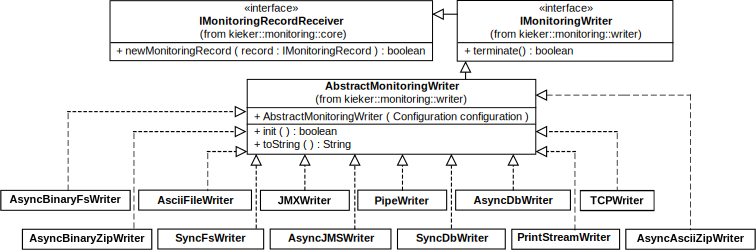
\includegraphics[scale=0.7]{images/kieker_writerimplsuserguide-modified}
		\caption{Interface \class{IMonitoringWriter} and some of the implementing classes}
		\label{figure:monitoringLogWritersHierarchy}
	\end{centering}
\end{figure}

Figure~\ref{figure:monitoringLogWritersHierarchy} shows some fo the monitoring writers %
already implemented in \KiekerMonitoringPart{}. The available properties for the %
included writers are well-documented in the %
example configuration file (see Appendix~\ref{sec:appdx:monitoringproperties}). %

% \enlargethispage{1.2cm}

Different writers can be used %
to store monitoring records to filesystems and databases respectively (e.g., \class{FileWriter}, \class{AsciiFileWriter}, %
\class{SyncFsWriter}, \class{AsyncDbWriter}, and \class{SyncDbWriter}). %
The variants with the prefix \class{Async} are implemented using asynchronous %
threads that decouple the I/O operations from the control flow of the %
instrumented application. %
As the new Kieker writer API uses always a fast pipe implementation to decouple the writer, nowadays all writers are asynchronuous.
Furthermore, the new \class{FileWriter} introduced new features and comes with a standard Kieker text serialization and a binary serialization.
In addition, it can be extended to write other formats.
The \class{AsciiFileWriter} is the default writer that has already been used in %
Section~\ref{sec:example:monitoring}. %
Please note that the database writers are currently in a prototype stage and
that they should be used with care. %
The \class{PrintStreamWriter} simply sends the String representation of incoming %
records to the standard output or standard error streams, which can be helpful %
for debugging purposes.

The \class{JmsWriter} and \class{JmxWriter} write records to a JMS %
(Java Messaging Service~\cite{JMS-WebSite}) queue and JMX (Java Management %
Extensions~\cite{JMX-Website}) queue respectively. The \class{PipeWriter} %
allows to pass records via in-memory record streams (named pipes). %
These writers allow to implement on-the-fly analysis in distributed systems, i.e., analysis while %
continuously receiving new monitoring data from an instrumented application potentially %
running on another machine. A more detailed description of how to use the \class{JmsWriter} %
can be found in Appendix~\ref{appendix:usingJMS}. %

\noindent Listing~\ref{listing:MyWriter} %on page~\pageref{listing:MyWriter} 
shows %
a custom writer \class{MyPipeWriter} which uses a named pipe to %
write the given records into a buffer located in the memory. The source code of %
the class \class{MyPipe} is listed in Appendix~\ref{appendix:pipeListings}. %

\setJavaCodeListing
\lstinputlisting[caption=MyPipeWriter.java, label=listing:MyWriter,firstline=23,firstnumber=23]{\customComponentsBookstoreApplicationDir/src/kieker/examples/userguide/ch3and4bookstore/MyPipeWriter.java}

% \pagebreak

\pagebreak

\noindent The monitoring writer to be used is selected by the %
\KiekerMonitoringPart{} configuration property (Section~\ref{chap:componentsMonitoring}) %
\textit{kieker.monitoring.writer}. Writer-specific configuration properties %
can be provided by properties prefixed by the fully-qualified writer classname.  %
Listing~\ref{lst:monitoringwriter:MyWriter} demonstrates how to use the custom %
writer \class{MyPipeWriter} defined above. In this example, the pipe name is %
passed as the property value \textit{pipeName}.

\setPropertiesListing
\lstinputlisting[caption={Configuration of the custom writer \class{MyPipeWriter}},label=lst:monitoringwriter:MyWriter,firstline=5,firstnumber=5,lastline=6]%
{\customComponentsBookstoreApplicationDir/src-resources/META-INF/kieker.monitoring.properties}

\enlargethispage{1cm}

\noindent As the data structure of this kind of monitoring stream, we created a %
class \class{PipeData} in order to demonstrate the use of the \method{toArray} and %
\method{initFromArray} (in Section~\ref{sec:analysis:reader}) methods. %
A \class{PipeData} object holds a logging timestamp and an \class{Object} array %
containing the serialized record data. %
Appendix~\ref{appendix:pipeListings} includes a source code listing of this class. %
Alternatively, we could have used \class{IMonitoringRecord} as the data structure %
used by the pipe. This is the way, \Kieker{}'s \class{PipeWriter} works. %

  %%%%%%%%%%%%%%%%%%%%%%%%%%%%%%%%%%%%%%%%%
% Kieker Analysis Component
%
% $Date$
% $Rev$:
% $Author$

\chapter{\KiekerAnalysisPart{} Component}\label{chap:componentsAnalysis}

\NOTIFYBOX{The Java sources of this chapter, as well as a pre-compiled binary, %
can be found in the %
\file{\customComponentsBookstoreApplicationReleaseDirDistro{}/} directory of the %
binary release.}

\section{Pipe-and-Filter Framework and Included Plugins}\label{sec:analysis:controller}

\KiekerAnalysisPart{} provides a framework to define and execute pipe-and-filter %
architectures of analysis plugins, i.e., monitoring readers and analysis filters, %
as well as repositories. %
This section describes how to use and develop readers, filters, and %
repositories. The description is based on the example %
pipe-and-filter architecture shown in Figure~\ref{fig:example:pipe-and-filter}. The custom monitoring reader %
\class{MyPipeReader}, which corresponds to the writer developed in Section~\ref{sec:monitoring-log-writers}, %
sends records to the connected custom filter \class{MyResponseTimeFilter}. %
This filter accepts only events of the record type \class{MyResponseTimeRecord},
developed in Section~\ref{sec:componentsMonitoring:monitoringRecords}. %
The \class{MyResponseTimeFilter} classifies incoming \class{MyResponseTimeRecord}s %
based on whether they satisfy or exceed a configured threshold and passes them %
to the respective output ports, \method{validResponseTimes} or \method{invalidResponseTimes}. %
Two instances of a second custom filter, \class{MyResponseTimeOutputPrinter}, %
print the received records to the standard output stream.

\begin{figure}
\includegraphics[width=\textwidth]{images/example-pipe-and-filter}
\caption{Example pipe-and-filter configuration}
\label{fig:example:pipe-and-filter}
\end{figure}

%  requires a monitoring reader %
% (Section~\ref{sec:analysis:reader}) and at least %
% one monitoring record consumer plugin (Section~\ref{sec:analysis:consumer}). %
% In addition to the monitoring record consumer plugin, %
% other analysis plugins can be registered. %

\begin{figure}\centering
\includegraphics[width=\textwidth]{images/kieker_AnalysisControlleruserguide-modified}
\caption{Class diagram showing important \KiekerAnalysisPart{} types and their relationship}
\label{fig:analysisController:classdiagram}
\end{figure}

% \pagebreak

\noindent Figure~\ref{fig:analysisController:classdiagram} shows the class diagram %
with the important \KiekerAnalysisPart{} classes and their relationships. %
Note that only the most important methods are included. 
An analysis with \KiekerAnalysisPart{} is set up and executed employing %
the class \class{AnalysisController}. %
Setting up and running an analysis with \KiekerAnalysisPart{} requires the %
following steps to be performed, as sketched in Section~\ref{sec:example:analysis} already:

\enlargethispage{1.2cm}

\medskip

\begin{compactenum}
\item Creating an instance of the \class{AnalysisController} class
\item Creating monitoring readers, filters, and repositories.
\item Connecting plugins to other plugins and to repositories (\method{connect})
\item Starting the analysis instance (\method{run}).
\end{compactenum}

\medskip

\noindent On invocation of the \method{run} method, the \class{AnalysisController} %
calls the \method{init} method of all filter plugins allowing them to initialize. %
Then, it starts the configured monitoring readers by calling its \method{read} %
method. Plugins send data via their output ports to connected input ports of other
plugins. Being the source in a pipe-and-filter architecture, readers don't have %
input ports. Plugins can be connected to repositories, which may provide %
shared services, such as managed access to a common architectural model %
of the analyzed system. As soon as all readers have returned from the execution of their \method{read}
methods, the method \method{terminate} of each registered plugin is called by the %
\class{AnalysisController}. \KiekerAnalysisPart{} configurations can be saved %
to a \class{.kax} file by calling the \class{AnalysisController}'s \method{saveToFile} method. %
The \class{AnalysisController} provides a constructor which accepts the %
file system location of a \class{.kax} file to load the configuration from. %
%See Appendix~\ref{appendix:wrapperScripts:kaxRun} and~\ref{appendix:wrapperScripts:kaxViz} %
%for included tools/scripts which execute and visualize \class{.kax} files.
 %
In order to support the asynchronous execution of the \class{AnalysisController} instance, %
we provide the \class{AnalysisControllerThread} class.

\subsection{Programmatic Creation of Pipe-and-Filter Architectures}\label{sec:analysis:programmaticCreation}

To give a first impression of the programmatic %
instantiation, configuration, and connection of plugins, Listing~\ref{listing:StarterInitConnect} %
demonstrates this procedure for the example, using \class{MyPipeReader} and %
\class{MyResponseTimeFilter}, according to Figure~\ref{fig:example:pipe-and-filter}.

The configuration for the \class{MyPipeReader} is created in lines~51--52. %
Using this configuration, the reader is created in line~53. Similarly, %
lines~56--62 initialize the \class{MyResponseTimeFilter}. The reader's output is connected %
to the filter's input in line~63. %
The entire programmatic creation of the pipe-and-filter architecture shown %
in Figure~\ref{fig:example:pipe-and-filter}, can be found in the example  %
file \file{Starter.java}.

\medskip

\setJavaCodeListing
\lstinputlisting[caption=Initializing and connecting the example reader and filter (Starter.java),label=listing:StarterInitConnect,firstline=47, lastline=63, firstnumber=47]%
{\customComponentsBookstoreApplicationDir/src/kieker/examples/userguide/ch3and4bookstore/Starter.java}

\enlargethispage{0.5cm}

\subsection{Monitoring Reader Plugins}

% Warning-tag for the reader-writer-thing
The monitoring readers are the direct counterpart to the monitoring %
writers. While writers receive records and write them into files or other kinds %
of monitoring logs/streams, readers deserialize monitoring data and provide it as %
\class{IMonitoringRecord} instances.

\begin{figure}\centering
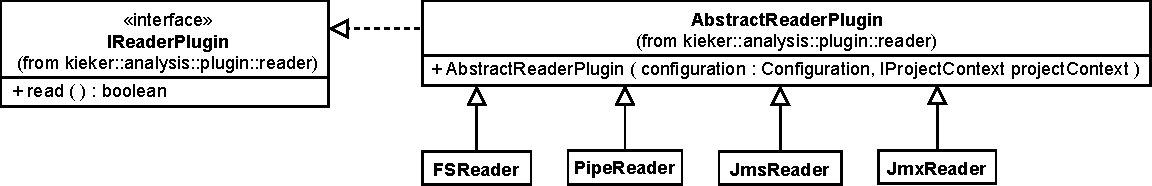
\includegraphics[scale=0.7]{images/kieker_readerimplsuserguide-modified}
\caption{Monitoring reader plugins included with \Kieker{}}
\label{Figure:ReaderHierarchy}
\end{figure}

% \pagebreak

% \
%
% \WARNBOX{This means that whenever a new writer is implemented, a corresponding reader has to be implemented as well. If one want for example to store the recorded informations in a database, one should be capable of reading these saved informations from the database again.}
%
% \

% \enlargethispage{1cm}

\noindent There are already some readers implemented in \Kieker,  as shown in the %
class diagram in Figure \ref{Figure:ReaderHierarchy}. %
The \class{FSReader} has already been used in Section~\ref{sec:example:analysis}. %
A brief description of how to use the \class{JmsReader} can be found in Appendix~%
\ref{appendix:usingJMS}. 
Like each plugin, readers are configured via properties, as used in Section~%
\ref{sec:analysis:programmaticCreation} and detailed in Section~%
\ref{sec:analysis:configuration}.

\subsection{Filter Plugins}

Filter plugins receive events (Java objects) via input ports from other %
plugins and implement analyses or visualizations based on these events. %
\Kieker{} already includes some basic filter plugins. For example, the %
\class{CountingFilter} and  \class{TeeFilter} forward incoming events %
to their output ports. The \class{CountingFilter} additionally provides the %
current number of received records via a second output port. The \class{TeeFilter} %
additionally prints incoming events to an output stream, which may be %
the standard output, standard error, a logger, or a file. %
A \class{TimestampFilter} and a \class{TypeFilter} filter incoming records by %
timestamp and by type, respectively. A \class{TraceIdFilter} filters incoming %
trace events (e.g., \class{OperationExecutionRecord}s, see Section~%
\ref{chap:example}) by trace ID. Additional filters for trace analysis, %
architecture reconstruction and visualization are included as part of %
the \KiekerTraceAnalysis{} tool, presented in Chapter~\ref{chap:aspectJ}. %
Like each plugin, filters are configured %
via properties, as used in Section~\ref{sec:analysis:programmaticCreation} and %
detailed in Section~%
\ref{sec:analysis:configuration}. %

% \pagebreak
% \setJavaCodeListing
%\lstinputlisting[caption=MyReponseTimeConsumer.java,label=lst:MyReponseTimeConsumer,firstline=21,firstnumber=21]{\customComponentsBookstoreApplicationDir/src/kieker/examples/userguide/ch3and4bookstore/MyResponseTimeConsumer.java}

% The following Listing~\ref{listing:AnalysisController} shows how to create and run an analysis %
% with these custom components:
%
% \setJavaCodeListing
% \lstinputlisting[caption=Code snippet setting up and running a \KiekerAnalysisPart{} instance (Starter.java),label=listing:AnalysisController,firstline=48, lastline=82, firstnumber=48]%
% {\customComponentsBookstoreApplicationReleaseDir/src/kieker/examples/userguide/ch3and4bookstore/Starter.java}

% \enlargethispage{1.2cm}

\subsection{Repositories}

Currently, \Kieker{} includes a single repository, \class{SystemModelRepository}, %
which is used by the \KiekerTraceAnalysis{} filters to update and query %
a component-based system model representing architectural entities %
and structures discovered while processing the incoming monitoring data. %
The development and use of repositories is detailed in Section~%
\ref{sec:analysis:repositories}. %

When using components of the \KiekerTraceAnalysis{}, make sure that write access to the %
\class{SystemModelRepository} is only triggered by readers. Some filters are terminated %
after the readers and expect the repository to be in a completed state.


\section{Developing Analysis Plugins and Repositories}\label{sec:analysis:plugins}

When implementing analysis plugins (i.e., readers or filters) and repositories, %
the classes \class{AbstractReaderPlugin}, \class{AbstractFilterPlugin}, or, %
respectively, \class{AbstractRepository} need to be extended %
(Figure~\ref{fig:analysisController:classdiagram}). %
Section~\ref{sec:analysis:configuration} describes how plugins and repositories %
can be configured via properties. %
Section~\ref{sec:analysis:pluginAnnotation} %
describes how to declare meta-information for plugins using %
dedicated annotations. %
Specific information on the development of custom filters, readers, and repositories %
are given in Sections~\ref{sec:analysis:filters}--\ref{sec:analysis:repositories}. %

% The monitoring record consumer plugins described in the following %
% Section~\ref{sec:analysis:consumer}, are special analysis plugins that receive %
% the monitoring records provided by the monitoring reader. %
% Starting with these monitoring record plugins, analysis plugins can be connected %
% in a pipe-and-filter style to implement more complex analyses. %
% \Kieker{} provides input and output port interfaces and implementing classes %
% to implement such analyses. See the documentation of the classes \class{AbstractInputPort} %
% and \class{OutputPort} for details. \KiekerTraceAnalysis{} is implemented %
% based on this pattern.

\subsection{Configuration}\label{sec:analysis:configuration}

\noindent According to the %
configuration of the \KiekerMonitoringPart{} components (see Section~\ref{sec:monitoring:configuration}),
plugins and repositories are configured via \class{Configuration} objects. Classes must %
provide a public constructor, accepting a \class{Configuration} and an \class{IProjectContext} (normally the \class{IAnalysisController} instance) object as %
its only arguments. It is important to invoke the constructor of the super class. %
The configuration properties accepted by a plugin or repository should be provided via \class{public static} %
constants with prefix \method{CONFIG\_PROPERTY\_NAME\_} in order to ease the %
programmatic initialization of plugins (Section~\ref{sec:analysis:programmaticCreation}). %
For the example filter \class{MyResponseTimeFilter},
Listing~\ref{listing:MyResponseTimeFilterConstructor} shows the constructor,
the configuration property, and the corresponding member value obtained from the %
configuration.

\setJavaCodeListing
\lstinputlisting[firstline=44, firstnumber=44, lastline=52, caption={Plugin constructor accepting a \class{Configuration} and an \class{IProjectContext} object}, label=listing:MyResponseTimeFilterConstructor]%
{\customComponentsBookstoreApplicationDir/src/kieker/examples/userguide/ch3and4bookstore/MyResponseTimeFilter.java}

\noindent Additionally, the %
current configuration must be provided via the method %
\method{getCurrentConfiguration}. Please note that the returned configuration %
should be sufficient to initialize the plugin or repository via the mentioned constructor. %
The \class{AnalysisController} uses the \method{getCurrentConfiguration} to %
save the pipe-and-filter configuration. Listing~\ref{listing:MyResponseTimeFilterEventsToOutput} %
shows how the methods are implemented for the example filter \class{MyResponseTimeFilter}. %

\enlargethispage{1cm}

\setJavaCodeListing
\lstinputlisting[firstline=69, firstnumber=69, lastline=74, caption={Plugin returning its current configuration}, label=listing:MyResponseTimeFilterEventsToOutput]%
{\customComponentsBookstoreApplicationDir/src/kieker/examples/userguide/ch3and4bookstore/MyResponseTimeFilter.java}

\noindent The declaration of the available properties and their default values within a plugin is shown in section~\ref{sec:analysis:pluginAnnotation}, as this is done with annotations.

% \pagebreak

\subsection{@Plugin Annotation and Output Ports}\label{sec:analysis:pluginAnnotation}

\noindent The \class{@Plugin} class annotation is used to define a %
plugin name, a description, and the lists of output ports and configuration %
properties with default values. %
Listing~\ref{listing:MyResponseTimeFilterPluginAnnotationOutputs} shows the %
\class{@Plugin} annotation for the example filter.

\enlargethispage{1cm}

If the \class{@Plugin} annotation is not present for a plugin, the \method{name} %
defaults to the plugin's (simple) classname, the \method{description} defaults %
to the empty string, and the list of output ports is empty. These default values %
are also used in case a respective attribute is omitted. %
Note that the name is not required to be a unique among filters; it is simply %
used for descriptive purposes, such as in Figure~\ref{fig:example:pipe-and-filter}. %

Output ports are specified using the nested \class{@OutputPort} annotation. %
In addition to a name and a description for the output port, a list of event %
types can be specified. Note that in this case, the name is mandatory and must %
be unique for a plugin, as it is used for connecting input and output ports. %
The list of event types defaults to a list including only \class{Object.class}. %
The output port names should be provided as a \class{public static} constant %
with prefix \method{OUTPUT\_PORT\_NAME\_}, in order to ease the programmatic %
connection of readers and filters, as described in %
Section~\ref{sec:analysis:programmaticCreation}. Repositories required by %
filters are also specified as part of the \class{@Plugin} annotation. %
This is detailed in Section~\ref{sec:analysis:repositories}. %

\setJavaCodeListing
\lstinputlisting[firstline=27, firstnumber=27, lastline=40, caption={@Plugin annotation for the example plugin \class{MyResponseTimeFilter}}, label=listing:MyResponseTimeFilterPluginAnnotationOutputs]%
{\customComponentsBookstoreApplicationDir/src/kieker/examples/userguide/ch3and4bookstore/MyResponseTimeFilter.java}

\noindent Plugins can send events to their output ports by calling the %
\method{deliver} method provided by the super class. The method expects the %
output port name and the event to be sent as arguments. Listing~%
\ref{listing:MyResponseTimeFilterDelivers} %
shows how the example filter plugin \class{MyResponseTimeFilter} delivers records %
to its two output ports declared in the \class{@Plugin} annotation.

% \pagebreak

\setJavaCodeListing
\lstinputlisting[firstline=61, firstnumber=61, lastline=65, caption={Plugin sending events to output ports}, label=listing:MyResponseTimeFilterDelivers]%
{\customComponentsBookstoreApplicationDir/src/kieker/examples/userguide/ch3and4bookstore/MyResponseTimeFilter.java}

Listing~\ref{listing:MyResponseTimeFilterPluginAnnotationOutputs} shows also how %
the properties are declared. Using the \class{@Property} annotation, it is possible to declare %
the existing properties. Each property has a default value which should be sufficient %
to initialize the plugin.%

The \class{@Plugin} annotation (as well as the later introduced \class{@Repository} annotation) contains %
furthermore the two fields \method{dependencies} and \method{programmaticOnly}. The first %
one offers the possibility to give a description of the needed dependencies for a plugin %
(other libraries e.g.). The latter marks whether the current plugin (or repository) is for %
programmatic purposes only, i.e., they are of little use in graphical analysis %
tools.

\subsection{Developing Monitoring Reader Plugins}\label{sec:analysis:reader}

\noindent Custom readers must extend the class %
\class{AbstractReaderPlugin} (see Figure~\ref{fig:analysisController:classdiagram}), %
and implement the methods \method{init}, \method{read}, and \method{terminate}, %
which are called by the \class{AnalysisController} to trigger the reader's initialization, %
reading, and termination. Like each plugin (Section~\ref{sec:analysis:configuration}), %
readers are configured via a constructor accepting a \class{Configuration} and an \class{IProjectContext} object %
as its only arguments; they must provide the current configuration %
via the implemented \method{getCurrentConfiguration} %
method. Readers start reading on invocation of the \method{read} method, %
providing the obtained records to connected filters via the output port(s) %
declared in the \class{@Plugin} annotation (Section~\ref{sec:analysis:pluginAnnotation}). %
The \method{read} method should be implemented synchronously, i.e., it should %
return after reading is finished or has been aborted via an invocation of the %
\method{terminate} method.

% If there is nothing on the pipe to be read, the reader waits 4 seconds at maximum before it terminates.
% \setJavaCodeListing
% \lstinputlisting[firstline=29, firstnumber=29, caption=MyPipeReader.java (excerpt), label=listing:MyReader,float]{\customComponentsBookstoreApplicationDir/src/kieker/examples/userguide/ch3and4bookstore/MyPipeReader.java}

\enlargethispage{1cm}

\setJavaCodeListing
\lstinputlisting[firstline=28, firstnumber=28, lastline=40, caption={@Plugin annotation for the example reader}, label=listing:MyPipeReaderPluginAnnotation]%
{\customComponentsBookstoreApplicationDir/src/kieker/examples/userguide/ch3and4bookstore/MyPipeReader.java}

Listing~\ref{listing:MyPipeReaderPluginAnnotation} shows the \class{@Plugin} %
annotation  of the example reader \class{MyPipeReader}. Reading monitoring %
records from the monitoring pipe introduced in the previous Chapter~%
\ref{sec:monitoring-log-writers}, the reader provides received monitoring %
records via its output port.

\noindent Listing~\ref{listing:MyPipeReaderInit} shows an excerpt of the \class{MyPipeReader}'s %
constructor. In this case, the reader reads the pipe name from the %
configuration and connects to the named pipe. Optionally, the reader can override the 
\method{init} method.

 \pagebreak

\setJavaCodeListing
\lstinputlisting[firstline=51, firstnumber=51, lastline=57, caption={Example reader's initialization in the constructor (excerpt)}, label=listing:MyPipeReaderInit]%
{\customComponentsBookstoreApplicationDir/src/kieker/examples/userguide/ch3and4bookstore/MyPipeReader.java}

% \pagebreak

\noindent Listing~\ref{listing:MyPipeReaderRead} shows the \class{MyPipeReader}'s %
\method{read} method. In this case, the reader polls the pipe for new records %
and forwards these to its output port.

\setJavaCodeListing
\lstinputlisting[firstline=60, firstnumber=60, lastline=80, caption={Example reader's \method{read} method}, label=listing:MyPipeReaderRead]%
{\customComponentsBookstoreApplicationDir/src/kieker/examples/userguide/ch3and4bookstore/MyPipeReader.java}

\vspace{-0.2cm}

\subsection{Developing Filter Plugins}\label{sec:analysis:filters}

Custom filters must extend the class \class{AbstractFilterPlugin}. %
In addition to providing meta information, including output ports, via the %
\class{@Plugin} annotation %
(Section~\ref{sec:analysis:pluginAnnotation}), as well as implementing a constructor %
and the getter for handling the \class{Configuration} (Section~\ref{sec:analysis:configuration}), %
filters may override the methods \method{init} and %
\method{terminate}, implementing initialization and cleanup tasks. %
The \class{@Plugin} annotation of the example filter \class{MyResponseTimeFilter} %
was shown in Listing~\ref{listing:MyResponseTimeFilterPluginAnnotationOutputs} already.

% \enlargethispage{1cm}

Filters receive events via methods marked with the \class{@InputPort} %
annotation. These methods must accept a single argument, which has to be %
a super type of the set of accepted event types declared in the respective %
\class{@InputPort} annotation's \method{eventTypes}. %
In addition to an optional \method{description}, each \class{@InputPort} %
must have a \method{name}, which is unique for this filter. The input port names %
should be provided as a \class{public static} constants %
with prefix \method{INPUT\_PORT\_NAME\_}, in order to ease the programmatic %
connection of readers and filters, as described in %
Section~\ref{sec:analysis:programmaticCreation}. %
Listing~\ref{listing:MyResponseTimeFilterInputPort} shows the declaration %
of the input port provided by the example plugin \class{MyResponseTimeFilter}. %
The body of this method was shown in Listing~%
\ref{listing:MyResponseTimeFilterDelivers} already.

% \pagebreak

\setJavaCodeListing
\lstinputlisting[firstline=56, firstnumber=56, lastline=60, caption={@InputPort annotation for the example plugin's input method}, label=listing:MyResponseTimeFilterInputPort]%
{\customComponentsBookstoreApplicationDir/src/kieker/examples/userguide/ch3and4bookstore/MyResponseTimeFilter.java}

\subsection{Developing and Accessing Required Repositories}\label{sec:analysis:repositories}

Custom repositories must extend the class \class{AbstractRepository}. %
The \class{@Repository} annotation is used to provide a \method{name} %
and a \method{description} for a repository type. %
Listing~\ref{listing:RepositoryAnnotation} shows the \class{@Repository} annotation %
of the \class{SystemModelRepository}, which is included in \Kieker{} as part of the %
\KiekerTraceAnalysis{} tool. %

\enlargethispage{1cm}

\setJavaCodeListing
\lstinputlisting[firstline=43, firstnumber=43, lastline=46, caption={\class{@Repository} annotation of Kieker's \class{SystemModelRepository}}, label=listing:RepositoryAnnotation]%
{../../kieker-tools/src/kieker/tools/trace/analysis/systemModel/repository/SystemModelRepository.java}

\noindent Plugins specify the list of required repositories in their %
\class{@Plugin} annotation. Repositories are connected to filter-provided %
repository ports. A plugin's repository ports are specified using the %
nested \class{@RepositoryPort} annotation, as depicted for a %
\KiekerTraceAnalysis{} filter in Listing~\ref{listing:RepositoryRequirementDeclaration}. %
Like for input and output port names, this name must be unique for the plugin %
and should be provided as a \class{public static} constant %
with prefix \method{REPOSITORY\_PORT\_NAME\_}, in order to ease the programmatic %
connection of repositories to readers and filters. %

\setJavaCodeListing
\lstinputlisting[firstline=40, firstnumber=40, lastline=41, caption={Declaration of required repositories in the @Repository annotation}, label=listing:RepositoryRequirementDeclaration]%
{../../kieker-tools/src/kieker/tools/trace/analysis/filter/AbstractTraceAnalysisFilter.java}

\pagebreak

\noindent Plugins can access their connected repositories via the \method{getRepository} %
method provided by the super class, as shown in Listing~\ref{listing:RepositoryAccess}. %

\setJavaCodeListing
\lstinputlisting[firstline=161, firstnumber=161, lastline=162, caption={Accessing a repository within a plugin}, label=listing:RepositoryAccess]%
{../../kieker-tools/src/kieker/tools/trace/analysis/filter/AbstractTraceAnalysisFilter.java}


%  %%%%%%%%%%%%%%%%%%%%%%%%%%%%%%%%%%%%%%%%%
% Trace Analysis and Monitoring
%
% $Date$
% $Rev$:
% $Author$

\chapter{\KiekerTraceAnalysis{} Tool}\label{chap:aspectJ}

\KiekerTraceAnalysis{} implements the special feature of \Kieker{} allowing to %
monitor, analyze, and visualize (distributed) traces of method executions and %
corresponding timing information. For this purpose, it includes monitoring probes employing %
AspectJ~\cite{AspectJ-WebSite}, Java~EE Servlet~\cite{JavaServletTechnology-WebSite}, %
Spring~\cite{Spring-WebSite}, and Apache~CXF~\cite{CXF-WebSite} technology. %
Moreover, it allows to reconstruct and visualize architectural models of the %
monitored systems, e.g., as sequence and dependency diagrams. %

Section~\ref{chap:example} already introduced parts of the monitoring record %
type \class{OperationExecutionRecord}. \KiekerTraceAnalysis{} uses this record %
type to represent monitored executions and associated trace and session information. %
Figure~\ref{fig:OperationExecutionRecordClassDiagramComplete} shows a class diagram %
with all attributes of the record type \class{OperationExecutionRecord}. %
The attributes \method{className}, \method{operationName}, %
\method{tin}, and \method{tout} have been introduced before. %
The attributes \method{traceId} and \method{sessionId} are used to store %
trace and session information; \method{eoi} and \method{ess} contain control-flow %
information needed to reconstruct traces from monitoring data. %
For details on this, please refer to our technical %
report~\cite{vanHoornRohrHasselbringWallerEhlersFreyKieselhorst2009TRContinuousMonitoringOfSoftwareServicesDesignAndApplicationOfTheKiekerFramework}.

\begin{figure}[hb]\centering
\includegraphics[scale=0.8]{images/kieker_OperationExecutionRecord-complete-modified}%
\caption{The class diagram of the operation execution record}
\label{fig:OperationExecutionRecordClassDiagramComplete}
\end{figure}

\enlargethispage{1cm}

\noindent Section~\ref{sec:traceMonitoring} describes how to instrument Java %
applications for monitoring trace information. %
It presents the technology-specific probes provided by \Kieker{} for this %
purpose---with a focus on AspectJ. %
Additional technology-specific probes can be implemented based on the existing %
probes. %
Section~\ref{sec:traceAnalysisTool} presents the %
tool which can be used to analyze and visualize the recorded trace %
data.  Examples for the available analysis and visualization outputs %
provided by \KiekerTraceAnalysis{} are presented in %
Section~\ref{sec:traceAnalysisExamples}.

\section{Monitoring Trace Information}\label{sec:traceMonitoring}

The following Sections describe how to use the monitoring probes based on %
AspectJ (Section~\ref{sec:traceAnalysis:instr:AspectJ}), %
the Java Servlet~API (Section~\ref{sec:traceAnalysis:instr:servlet}), %
the Spring Framework (Section~\ref{sec:traceAnalysis:instr:spring}), and %
Apache~CXF (Section~\ref{sec:traceAnalysis:instr:cxf}) provided %
by \Kieker{}. %

\subsection{AspectJ-Based Instrumentation}\label{sec:traceAnalysis:instr:AspectJ}

AspectJ~\cite{AspectJ-WebSite} allows to weave code into the byte code of %
Java applications and libraries without requiring manual modifications of the %
source code. %
\Kieker{} includes the AspectJ-based monitoring probes %
\class{OperationExecutionAspectAnnotation}, %
\class{OperationExecutionAspectAnnotationServlet}, %
\class{OperationExecutionAspectFull}, and %
\class{OperationExecutionAspectFullServlet} %
which can be woven into Java applications at compile time and load time. %
These probes monitor method executions and corresponding %
trace and timing information. The probes with the postfix \class{Servlet} %
additionally store a session identifier within the \class{OperationExecutionRecord}. %
When the probes with name element \class{Annotation} are used, %
methods to be monitored must be annotated by the \Kieker{} %
annotation \class{@OperationExecutionMonitoringProbe}. %
This section demonstrates how to use the AspectJ-based probes to monitor %
traces based on the Bookstore application from Chapter~\ref{chap:example}. %

% \enlargethispage{1.0cm}

\NOTIFYBOX{The Java sources of the example presented in %
this section, as well as a pre-compiled binary, can be found in the %
\file{\aspectJBookstoreApplicationReleaseDirDistro{}/} directory of the %
binary release.}

% \

% This chapter will show in Section~\ref{sec:aspectJ:annotation} how
% to use AspectJ to mark methods to be monitored with a simple annotation
% in order to avoid the manual monitoring as seen in Chapter~\ref{chap:example}
% and \ref{chap:componentsMonitoring}. Once the methods are marked, the AspectJ-Weaver-Agent
% will surround the calls with the necessary code during runtime, similar
% to the manually inserted instrumentation code used in Section~\ref{sec:example:monitoring}.
% An alternative solution will be shown as well in Section~\ref{sec:aspectJ:fullweaving}, %
% where the methods to be instrumented are specified using an external configuration file %
% without requiring source code modifications. Both solutions
% can be used to reconstruct architectural views and to perform trace
% analyses. The result of both will be diagrams similar to sFigure~\ref{fig:bookstore:classAndSequenceDiagrams}.

% The idea of weaving the monitoring-code into the ``plain'' code
% during compile-time seems to suggest itself, but
% in this chapter it
% is only shown how to perform the so called load-time-weaving - the
% weaving during runtime.%, which is more flexible than the compile-time-weaving.

\begin{figure}[H]
\begin{graybox}
\dirtree{%
.1 \DirInDirTree{examples/}. %\DTcomment{The root directory of the project}.
.2 \DirInDirTree{userguide/}.
.3 \DirInDirTree{ch5--trace-monitoring-aspectj/}.
.4 \DirInDirTree{build/}\DTcomment{Directory for the Java class files}.
.5 \DirInDirTree{libs/}.
.6 BookstoreApplication.jar.
.4 \DirInDirTree{gradle/}.
.5 \DirInDirTree{wrapper/}\DTcomment{Directory for the gradle wrapper}.
.6 \ldots.
.4 \DirInDirTree{lib/} \DTcomment{Directory for the needed libraries}.
.5 \newFileDirInDirTree{\mainJarWeaver}.
.4 \DirInDirTree{src/}\DTcomment{Directory for the source code files}.
.5 \DirInDirTree{../ch5bookstore/}.
.6 Bookstore.java.
.6 BookstoreHostnameRewriter.java.
.6 BookstoreStarter.java.
.6 Catalog.java.
.6 CRM.java.
.4 \DirInDirTree{src-resources/}.
.5 \DirInDirTree{META-INF/}\DTcomment{Directory for the configuration files}.
.6 aop.xml.
.6 aop-event.xml.
.6 aop-full.xml.
.6 kieker.monitoring.adaptiveMonitoring.conf.
.6 \kiekerMonitoringProperties{}. 
.3 build.gradle.
.3 gradlew.
.3 gradlew.bat.
.3 README.txt.
}
\end{graybox}

\caption{The new directory structure of the Bookstore application}
\label{fig:bookstoreAOP:dirStructure}
\end{figure}

Figure~\ref{fig:bookstoreAOP:dirStructure} shows the directory used by the example of this section. %
The jar-file \file{\mainJarWeaver} already includes the \textit{AspectJ weaver}, %
which is registered with the JVM and weaves the monitoring instrumentation into %
the Java classes. It will be configured based on the configuration file %
\file{\file{\aopConfigFile}}, for which a working sample file is provided in the %
example's \dir{META-INF/} directory. Instead of registering the \file{\mainJarWeaver} %
as an agent to the JVM, the \file{\aspectJWeaverJar} can be used. In this case, %
the \file{\mainJar} needs to be added to the classpath.

\pagebreak

Once the necessary files have been copied to the example directory, the source code can be instrumented with the annotation
\class{OperationExecutionMonitoringProbe}. Listing~\ref{lst:BookstoreAspectJ} shows how the annotation is used.

\setJavaCodeListing
\lstinputlisting[caption=Bookstore.java, label=lst:BookstoreAspectJ,firstline=21,firstnumber=21]{\aspectJBookstoreApplicationDir/src/kieker/examples/userguide/ch5bookstore/Bookstore.java}

\noindent As a first example, each method of the Bookstore application will be annotated. The annotation can be used to instrument all methods except for constructors.

The \file{\aopConfigFile} file has to be modified to specify the classes to be considered for instrumentation by the AspectJ weaver. Listing~\ref{lst:aopConfigFileAnnotations} shows the modified configuration file.

\enlargethispage{1cm}
\setXMLListing
\lstinputlisting[caption=aop.xml, label=lst:aopConfigFileAnnotations]{\aspectJBookstoreApplicationDir/src-resources/META-INF/aop.xml}

\noindent Line~5 tells the AspectJ weaver to consider all classes inside the example package. %
AspectJ allows to use wild-cards for the definition of classes to %
include---e.g., \lstinline$<include within="bookstoreTracing.Bookstore*"/>$ to weave all %
classes with the prefix \class{Bookstore} located in a package \class{bookstoreTracing}.

Line~9 specifies the aspect to be woven into the classes. In this case, the \Kieker{} %
probe \class{OperationExecutionAspectAnnotation} is used. It requires that %
methods intended to be instrumented are annotated by %
\lstinline[language=Java]{@OperationExecutionMonitoringProbe}, as mentioned before.

Listings~\ref{lst:traceAnalysisCompileRunExample1} and %
\ref{lst:traceAnalysisCompileRunExample1Win} show how to compile and run the annotated %
Bookstore application. The \file{\aopConfigFile} must be located in a %
\dir{META-INF/} directory in the classpath---in this case the \dir{build/} directory. %
The AspectJ weaver has to be loaded as a so-called Java-agent. It weaves the %
monitoring aspect into the byte code of the Bookstore application. %
Additionally, a \file{\kiekerMonitoringProperties{}} is copied to the \dir{META-INF/} directory. %
This configuration file may be adjusted as desired (see Section~\ref{sec:monitoring:configuration}).

\


\setBashListing
\input{ch5-trace-analysis_Compile_Run_Example_1.inc}
\input{ch5-trace-analysis_Compile_Run_Example_1.inc-win}

\noindent After a complete run of the application, the monitoring files should appear in %
the same way as mentioned in Section~\ref{sec:example:monitoring} including the %
additional trace information. An example log of a complete run can be found in %
Appendix~\ref{sec:appendix:exampleConsoleOutputs:aspectJExample}.

\paragraph*{Instrumentation without annotations}%\label{sec:aspectJ:fullweaving}

AspectJ-based instrumentation without using annotations is quite simple. It is %
only necessary to modify the file \file{\aopConfigFile{}}, as shown %
in Listing~\ref{lst:aopConfigFileFull}.
\pagebreak
\setXMLListing
\lstinputlisting[caption=aop.xml, label=lst:aopConfigFileFull]{\aspectJBookstoreApplicationDir/src-resources/META-INF/aop-full.xml}

\noindent The alternative aspect \class{OperationExecutionAspectFull} is being %
activated in line~9. As indicated by its name, this aspect makes sure that every %
method within the included classes/packages will be instrumented and monitored. %
% The exact behavior can be controlled very exactly by using appropriate includes and excludes within the weaver-part of the configuration file. %
% For example,
Listing \ref{lst:aopConfigFileFull} demonstrates how to limit the %
instrumented methods to those of the class \class{BookstoreStarter}.

The commands shown in the Listings~\ref{lst:traceAnalysisCompileRunExample1} and %
\ref{lst:traceAnalysisCompileRunExample1Win} can again be used to compile and execute %
the example. Note that the annotations within the source code have no effect %
when using this aspect.

\

\WARNBOX{When using a custom aspect, it can be necessary to specify its %
classname in the \lstinline{include} directives of the \aopConfigFile{}.}

\subsection{Servlet Filters}\label{sec:traceAnalysis:instr:servlet}

The Java Servlet API~\cite{JavaServletTechnology-WebSite} includes the %
\class{javax.servlet.Filter} interface. It can be used to implement %
interceptors for incoming HTTP requests. %
\Kieker{} includes the probe %
\class{SessionAndTraceRegistrationFilter} which implements the %
\class{javax.servlet.Filter} interface. %
It initializes the session and trace information for incoming requests. %
If desired, it additionally creates an \class{OperationExecutionRecord} for each %
invocation of the filter and passes it to the \class{MonitoringController}.

% \enlargethispage{1.5cm}

Listing~\ref{lst:OperationExecutionRegistrationAndLoggingFilterInWebXML} %
demonstrates how to integrate the \class{SessionAndTraceRegistrationFilter} %
in the \file{web.xml} file of a web application.

The Java~EE Servlet container example described in Appendix~\ref{appendix:JavaEEServletExample} employs the %
\class{SessionAndTraceRegistrationFilter}.

\pagebreak

\setXMLListing
\lstinputlisting[firstline=50,lastline=61,firstnumber=50,%
caption=\class{SessionAndTraceRegistrationFilter} in a \file{web.xml} file,%
label=lst:OperationExecutionRegistrationAndLoggingFilterInWebXML]%
{\JavaEEServletExampleDir/jetty/webapps/jpetstore/WEB-INF/web.xml}


\subsection{Spring}\label{sec:traceAnalysis:instr:spring}

The Spring framework~\cite{Spring-WebSite} provides interfaces for intercepting %
Spring services and web requests. %
\Kieker{} includes the probes %
\class{OperationExecutionMethodInvocationInterceptor} and
\class{OperationExecutionWebRequestRegistrationInterceptor}. %
The \class{OperationExecutionMethodInvocationInterceptor} is similar to the %
AspectJ-based probes described in the previous section and monitors method %
executions as well as corresponding trace and session information. %
The \class{OperationExecutionWebRequestRegistrationInterceptor} intercepts %
incoming Web requests and initializes the trace and session data for this %
trace. If you are not using the \class{OperationExecutionWebRequestRegistrationInterceptor}, %
you should use one of the previously described Servlet filters to register %
session information for incoming requests %
(Section~\ref{sec:traceAnalysis:instr:servlet}).

See the Spring documentation for instructions how to add the interceptors %
to the server configuration.

\subsection{CXF SOAP Interceptors}\label{sec:traceAnalysis:instr:cxf}

The Apache~CXF framework~\cite{CXF-WebSite} allows to implement interceptors for web service calls, %
for example, based on the SOAP web service protocol. %
\Kieker{} includes the probes %
\class{OperationExecutionSOAPRequestOutInterceptor}, %
\class{OperationExecutionSOAPRequestInInterceptor}, %
\class{OperationExecutionSOAPResponseOutInterceptor}, and %
\class{OperationExecutionSOAPResponseInInterceptor} which can be used to %
monitor SOAP-based web service calls. %
Session and trace information is written to and read from the SOAP header of %
service requests and responses allowing to monitor distributed traces. %
See the CXF documentation for instructions how to add the interceptors %
to the server configuration.

\pagebreak

\section{Trace Analysis and Visualization}\label{sec:traceAnalysisTool}

\enlargethispage{0.5cm}

Monitoring data including trace information can be analyzed and visualized with the \KiekerTraceAnalysis{} tool which is included in the \Kieker{} binary as well.\\

\WARNBOX{
In order to use this tool, it is necessary to install two third-party programs:
\begin{enumerate}
\item \textbf{Graphviz} A graph visualization software which can be downloaded from \url{http://www.graphviz.org/}.
\item \textbf{GNU PlotUtils} A set of tools for generating 2D plot graphics which can be downloaded from \url{http://www.gnu.org/software/plotutils/} (for Linux) and from \url{http://gnuwin32.sourceforge.net/packages/plotutils.htm} (for Windows).
\item \textbf{ps2pdf} The \file{ps2pdf} tool is used to convert ps files to pdf files.
\end{enumerate}
Under Windows it is recommended to add the \dir{bin/} directories of both tools to the ``path'' environment variable. It is also possible that the GNU PlotUtils are unable to process sequence diagrams. In this case it is recommended to use the Cygwin port of PlotUtils.
}

\vspace{1mm}

\noindent Once both programs have been installed, the \KiekerTraceAnalysis{} tool can be used. It can be accessed via the wrapper-script \file{trace-analysis.sh} or \file{trace-analysis.bat} (Windows) in the \dir{bin/} directory. Non-parameterized calls of the scripts print all possible options on the screen. %, as listed in Appendix~\ref{appendix:wrapperScripts:traceAnalysis}.

The commands shown in Listings~\ref{lst:traceAnalysis:sequenceDiagram} and \ref{lst:traceAnalysis:sequenceDiagramWin} generate a sequence diagram as well as a call tree to an existing directory named \dir{out/}. The monitoring data is assumed to be located in the directory \dir{/tmp/kieker-20110428-142829399-UTC-Kaapstad-KIEKER/} or \dir{\%temp\%$\backslash{}$kieker-20100813-121041532-UTC-virus-KIEKER} under Windows. %

\setBashListing
\begin{lstlisting}[caption=Commands to produce the diagrams under \UnixLikeSystems,label=lst:traceAnalysis:sequenceDiagram]
#\lstshellprompt{}# #\textbf{./trace-analysis.sh}# #\textbf{--inputdirs}# /tmp/kieker-20110428-142829399-UTC-Kaapstad-KIEKER
                     #\textbf{--outputdir}# out/
                     #\textbf{--plot-Deployment-Sequence-Diagrams}#
                     #\textbf{--plot-Call-Trees}#
		     #\textbf{--short-labels}#
\end{lstlisting}

\begin{lstlisting}[caption=Commands to produce the diagrams under Windows,label=lst:traceAnalysis:sequenceDiagramWin]
#\lstshellprompt{}# #\textbf{trace-analysis.bat}# #\textbf{--inputdirs}# %temp%\kieker-20100813-121041532-UTC-virus-KIEKER
                    #\textbf{--outputdir}# out\
                    #\textbf{--plot-Deployment-Sequence-Diagrams}#
                    #\textbf{--plot-Call-Trees}#
		    #\textbf{--short-labels}#
\end{lstlisting}


\enlargethispage{1cm}

\WARNBOX{%
The Windows \file{.bat} wrapper scripts (including \file{trace-analysis.bat}) must be executed from within %
the \dir{bin/} directory.
}

\pagebreak

The resulting contents of the \dir{out/} directory should be similar to %
the following tree:

\begin{figure}[H]
\begin{graybox}
\dirtree{%
.1 \DirInDirTree{out/}.
.2 deploymentSequenceDiagram-6120391893596504065.pic.
.2 callTree-6120391893596504065.dot.
.2 system-entities.html.
}
\end{graybox}
\end{figure}

\noindent The \file{.pic} and \file{.dot} files can be converted into other formats, %
such as \file{.pdf}, by using the \textit{Graphviz} and \textit{PlotUtils} tools %
\file{dot} and \file{pic2plot}. %
The following Listing~\ref{lst:traceAnalysis:convertDiagrams} demonstrates this. %

% The generated diagrams are shown in the following %
% Figures~\ref{fig:traceAnalysis:callTree} and~\ref{fig:traceAnalysis:allocSeqDiagr}.

\input{ch5-trace-analysis_Convert_Diagrams.inc}

% \begin{figure}[H]\centering
%   \subfigure[]{\label{fig:traceAnalysis:callTree}%
%   \includegraphics[height=0.4\textheight]{images/callTree}
%   }%
%   \subfigure[]{\label{fig:traceAnalysis:allocSeqDiagr}%
%   \includegraphics[height=0.4\textheight]{images/allocationSequenceDiagram}
%   }%
%
%   \caption{Call Tree~\subref{fig:traceAnalysis:callTree} and Allocation Sequence Diagram~\subref{fig:traceAnalysis:allocSeqDiagr}}
% \end{figure}

\NOTIFYBOX{The scripts \file{dotPic-fileConverter.sh} and \file{dotPic-fileConverter.bat} %
convert all \file{.pic} and \file{.dot} in a specified directory. %
%See Appendix~\ref{appendix:wrapperScripts:dotPicFileConverter} for details.
}

\vspace{5mm}

Examples of all available visualization are presented in the following %
Section~\ref{sec:traceAnalysisExamples}.

\pagebreak

\section{Example \KiekerTraceAnalysis{} Outputs}\label{sec:traceAnalysisExamples}
\input{ch5-trace-analysis-exampleOutputs.inc}


  %%%%%%%%%%%%%%%%%%%%%%%%%%%%%%%%%%%%%%%%%
% Appendix
% 
% $Date$
% $Rev$:
% $Author$

\newpage
\appendix

% \chapter*{Appendix}\label{appendix}
\phantomsection
\addtocontents{toc}{\protect\pagebreak}
\addcontentsline{toc}{chapter}{Appendix}\hypertarget{hypertarget:appendix}{}
\addtocontents{toc}{\protect\setcounter{tocdepth}{0}}

\chapter{Wrapper Scripts}\label{appendix:wrapperScripts}
Please refer to the Kieker wiki under Kieker Tools.

\chapter{Java~EE Servlet Container Example}\label{appendix:JavaEEServletExample}
\input{Appendix-ch-javaEEServletContainerExample.inc}

\chapter{Using the JMS Writer and Reader}\label{appendix:usingJMS}
This chapter gives a brief description on how to use the \class{AsyncJmsWriter} and \class{JmsReader} %
classes. The directory \dir{\JMSBookstoreApplicationReleaseDirDistro/} contains the %
sources, gradle scripts etc.\ used in this example. It is based on the Bookstore %
application with manual instrumentation presented in Chapter~\ref{chap:example}. %

The following sections provide step-by-step instructions for the %
ActiveMQ JMS server implementation (Section~\ref{example:jms:activemq}).
The general procedure for this example is the following:

\medskip

\begin{compactenum}
 \item Download and prepare the respective JMS server implementation
 \item Copy required libraries to the example directory
 \item Start the JMS server
 \item Start the analysis instance which receives records via JMS
 \item Start the monitoring instance which sends records via JMS
\end{compactenum}

\

\WARNBOX{\quad\\Due to a bug in some JMS servers, avoid paths including white spaces.}

\section{ActiveMQ}\label{example:jms:activemq}

\subsection{Download and Prepare ActiveMQ}

Download an ActiveMQ archive from \url{http://activemq.apache.org/download.html}
and decompress it to the base directory of the example. Note, that there are two different %
distributions, one for Unix/Linux/Cygwin and another one for Windows, and that the latest supported version of ActiveMQ compatible with Java 7 is 5.14.5. 

Under \UnixLikeSystems{}, you'll need to set the executable-bit of the start script:

\setBashListing
\begin{lstlisting}[caption=]
 #\lstshellprompt{}# chmod +x bin/activemq
\end{lstlisting}

\noindent Also under \UnixLikeSystems{}, make sure that the file \file{bin/activemq} %
includes UNIX line endings (e.g., using your favorite editor or the \textit{dos2unix} tool).

\subsection{Copy ActiveMQ Libraries}

Copy the following files from the ActiveMQ release to the %
\dir{lib/} directory of this example:

\medskip

\enlargethispage{0.5cm}

\begin{compactenum}
\item \file{activemq-all-<version>.jar} (from ActiveMQ's base directory)
\item \file{slf4j-log4j<version>.jar} (from ActiveMQ's \dir{lib/optional} directory)
\item \file{log4j-<version>.jar} (from ActiveMQ's \dir{lib/optional} directory)
\end{compactenum}

\subsection{Kieker Monitoring Configuration for ActiveMQ}

The file \file{src-resources/META-INF/kieker.\-monitoring.\-pro\-perties-activeMQ} %
is already configured to use the \class{JmsWriter} via ActiveMQ. The important properties are %
the definition of the provider URL and the context factory:

\setPropertiesListing
\lstinputlisting[firstline=12,lastline=12,caption=Excerpt from \file{kieker.monitoring.properties-activemq} configuring the provider URL of the JMS writer via ActiveMQ]{\JMSBookstoreApplicationDir/src-resources/META-INF/kieker.monitoring.properties-activemq}

\setPropertiesListing
\lstinputlisting[firstline=21,lastline=21,caption=Excerpt from \file{kieker.monitoring.properties-activemq} configuring the context factory of the JMS writer via ActiveMQ]{\JMSBookstoreApplicationDir/src-resources/META-INF/kieker.monitoring.properties-activemq}

\subsection{Running the Example}

% \paragraph*{Execution}%
 The execution of the example is performed by the following three steps:
\begin{enumerate}
\item Start the JMS server (you may have to set your \class{JAVA\_HOME} variable first):

\setBashListing
\begin{lstlisting}[caption=Start of the JMS server under UNIX-like systems]
#\lstshellprompt{}# bin/activemq start
\end{lstlisting}
\begin{lstlisting}[caption=Start of the JMS server under Windows]
#\lstshellprompt{}# bin\#activemq start
\end{lstlisting}
\item Start the analysis part (in a new terminal):
\setBashListing
\begin{lstlisting}[caption=Start the analysis part under UNIX-like systems]
#\lstshellprompt{}# ./gradlew runAnalysisActiveMQ
\end{lstlisting}
\begin{lstlisting}[caption=Start the analysis part under Windows]
#\lstshellprompt{}# gradlew.bat runAnalysisActiveMQ
\end{lstlisting}
\item Start the instrumented Bookstore (in a new terminal):
\setBashListing
\begin{lstlisting}[caption=Start the analysis part under UNIX-like systems]
#\lstshellprompt{}# ./gradlew runMonitoringActiveMQ
\end{lstlisting}
\begin{lstlisting}[caption=Start the analysis part under Windows]
#\lstshellprompt{}# gradlew.bat runMonitoringActiveMQ
\end{lstlisting}
\end{enumerate}


\chapter{Using the AMQP Writer and Reader}\label{appendix:usingAMQP}
This chapter gives a brief description on how to use the \class{AmqpWriter} and \class{AmqpReader} %
classes, which allow to use Kieker with AMQP-based queue implementations such as %
RabbitMQ.\footnote{\url{http://www.rabbitmq.com}} The directory \dir{\AMQPBookstoreApplicationReleaseDirDistro/} %
contains the sources, gradle scripts etc.\ used in this example. It is based on the Bookstore %
application with manual instrumentation presented in Chapter~\ref{chap:example}. %

The following paragraphs provide step-by-step instructions for the popular AMQP implementation RabbitMQ.%

\section{Preparation}

\subsection{Download and Install RabbitMQ}
Download the RabbitMQ distribution from \url{http://www.rabbitmq.com/download.html} and follow the installation %
instructions for your OS. Since RabbitMQ requires Erlang, additional software packages may have to be installed %
on your machine.
\par In order to use RabbitMQ's integrated management UI, you may have to enable the appropriate plugin first. This is %
done by issuing the following command from the command line. 

\setBashListing
\begin{lstlisting}[caption=Enable the management UI under UNIX-like systems]
#\lstshellprompt{}# rabbitmq-plugins enable rabbitmq_management
\end{lstlisting}
\begin{lstlisting}[caption=Enable the management UI under Windows]
#\lstshellprompt{}# rabbitmq-plugins enable rabbitmq_management
\end{lstlisting}

Once the UI is enabled, you may access it at port 15672 by default. %

\subsection{Configure RabbitMQ}
Once the RabbitMQ server is installed and started, create a queue for Kieker to use. This can be done easily using %
RabbitMQ's management UI. It is accessible via \url{http://localhost:15672} (the default credentials are \texttt{guest:guest}) We will assume a queue named \parameterValue{kieker} for the remainder of this %
example. Please note the following caveats when configuring the server:

\begin{compactenum}
 \item If you choose to create a transient queue, the entire queue (not just the queued messages) is destroyed %
 on server shutdown and must be re-created manually. %
 \item The RabbitMQ server's default permissions grant access only from \hostname{localhost}. If your RabbitMQ server runs %
 on a remote machine, you have to set the permissions accordingly. %
\end{compactenum}

\subsection{Kieker Monitoring Configuration for RabbitMQ}
The file \file{src-resources/META-INF/kieker.\-monitoring.\-pro\-perties} %
is already configured to use the \class{AMQPWriter}. The important properties are %
the server URI and the queue name. %

\setPropertiesListing
\lstinputlisting[firstline=9,lastline=9,caption=Excerpt from \file{kieker.monitoring.properties} configuring the URI of the AMQP server]{\AMQPBookstoreApplicationDir/src-resources/META-INF/kieker.monitoring.properties}

\setPropertiesListing
\lstinputlisting[firstline=15,lastline=15,caption=Excerpt from \file{kieker.monitoring.properties} configuring the AMQP queue name]{\AMQPBookstoreApplicationDir/src-resources/META-INF/kieker.monitoring.properties}

\section{Running the Example}
The execution of the example is performed by the following three steps:
\begin{enumerate}
\item Ensure that the RabbitMQ server is started and the configured queue is accessible.

\item Start the analysis part (in a new terminal):
\setBashListing
\begin{lstlisting}[caption=Start the analysis part under UNIX-like systems]
#\lstshellprompt{}# ./gradlew runAnalysisAMQP
\end{lstlisting}
\begin{lstlisting}[caption=Start the analysis part under Windows]
#\lstshellprompt{}# gradlew.bat runAnalysisAMQP
\end{lstlisting}
\item Start the instrumented Bookstore (in a new terminal):
\setBashListing
\begin{lstlisting}[caption=Start the analysis part under UNIX-like systems]
#\lstshellprompt{}# ./gradlew runMonitoringAMQP
\end{lstlisting}
\begin{lstlisting}[caption=Start the analysis part under Windows]
#\lstshellprompt{}# gradlew.bat runMonitoringAMQP
\end{lstlisting}
\end{enumerate}

\chapter{Sigar-Based Samplers for System-Level Monitoring}\label{appendix:SigarBasedSamplers}
This chapter gives a brief description on how to use the included %
periodic samplers (Section~\ref{sec:componentsMonitoring:monitoringController:periodicSamplers}) %
for monitoring CPU utilization and memory/swap usage. %
The directory \dir{\SigarExampleReleaseDirDistro/} contains the %
sources, gradle scripts etc.\ used in this example. %
These samplers employ the Sigar API~\cite{HypericSigarWebsite}. \\%

\section{Preparation}

\begin{compactenum}
\item Copy the files \file{\mainJarEMF} and \file{\sigarJar} from the %
binary distribution to the example's \dir{lib/} directory.
\item Additionally, depending on the underlying system platform, %
corresponding Sigar native libraries need to be placed in the example's \dir{lib/} directory. %
Kieker's \dir{lib/sigar-native-libs/} folder already includes the right libraries for 32 and 64~bit Linux/Windows platforms. %
Native libraries for other platforms can be downloaded from~\cite{HypericSigarWebsite}. %
\end{compactenum}

\section{Using the Sigar-Based Samplers}

\WARNBOX{
	Using a very short sampling period with Sigar ($< 500$ ms) can result in monitoring log entries with NaN values. 
}

The Sigar API~\cite{HypericSigarWebsite} provides access to a number of system-level inventory and monitoring data, %
e.g., regarding memory, swap, cpu, file system, and network devices. %
Kieker includes Sigar-based samplers %
for monitoring CPU utilization %
(\class{CPUsDetailedPercSampler}, \class{CPUsCombinedPercSampler}) %
and memory/swap usage (\class{MemSwapUsageSampler}). %
When registered as a periodic sampler (Section~\ref{sec:componentsMonitoring:monitoringController:periodicSamplers}), %
these samplers collect the data of interest employing the Sigar API, %
and write monitoring records of types \class{CPUUtilizationRecord}, %
\class{ResourceUtilizationRecord}, and \class{MemSwapUsageRecord} respectively %
to the configured monitoring log/stream. %

Listing~\ref{listing:sigarSamplerMonitoringStarterExample} shows an excerpt from %
this example's \class{MonitoringStarter} %
which creates and registers two Sigar-based peridioc samplers. %
For reasons of performance and thread-safety, the \class{SigarSamplerFactory} %
should be used to create instances of the Sigar-based Samplers. 

%\pagebreak

\setJavaCodeListing
\lstinputlisting[firstline=38, lastline=51, firstnumber=38, caption=Excerpt from MonitoringStarter.java, label=listing:sigarSamplerMonitoringStarterExample]{\SigarExampleDir/src/kieker/examples/userguide/appendixSigar/MonitoringStarter.java}

\noindent Based on the existing samplers, users can easily create custom Sigar-based %
samplers by extending the class \class{AbstractSigarSampler}. For example, Listing~%
\ref{listing:sigarSamplerMethod} in Section~\ref{sec:componentsMonitoring:monitoringController:periodicSamplers} %
shows the \class{MemSwapUsageSampler}'s \method{sample} method. %
Typically, it is also required to define a corresponding monitoring record type, %
as explained in Section~\ref{sec:componentsMonitoring:monitoringRecords}. %
When implementing custom Sigar-based samplers, the \class{SigarSamplerFactory}'s \method{getSigar} method should %
be used to retrieve a \class{Sigar} instance. %

This example uses a stand-alone Java application to set up %
a Sigar-based monitoring process. When using servlet containers,  %
users may consider implementing this routine as a \class{ServletContextListener}, %
which are executed when the container is started and shutdown. %
As an example, Kieker includes a \class{CPUMemUsageServletContextListener}. %

\section{Executing the Example}

The execution of the example is performed by the following two steps:\\

\begin{compactenum}
\item Monitoring CPU utilization and memory usage for 30~seconds (class \class{MonitoringStarter}):
\setBashListing
\begin{lstlisting}[caption=Start of the monitoring under UNIX-like systems]
#\lstshellprompt{}# #\textbf{./gradlew}# runMonitoring
\end{lstlisting}
\begin{lstlisting}[caption=Start of the monitoring under Windows]
#\lstshellprompt{}# #\textbf{gradlew.bat}# runMonitoring
\end{lstlisting}

Kieker's console output lists the location of the directory containing the file system %
monitoring log. The following listing shows an excerpt: %

%\enlargethispage{1.5cm}
\pagebreak
\setBashListing
\begin{lstlisting}
 Writer: 'kieker.monitoring.writer.filesystem.AsciiFileWriter'
     Configuration:
             kieker.monitoring.writer.filesystem.AsciiFileWriter.QueueFullBehavior='0'
             kieker.monitoring.writer.filesystem.AsciiFileWriter.QueueSize='10000'
             kieker.monitoring.writer.filesystem.AsciiFileWriter.customStoragePath=''
             kieker.monitoring.writer.filesystem.AsciiFileWriter.storeInJavaIoTmpdir='true'
     Writer Threads (1): 
             Finished: 'false'; Writing to Directory: '/tmp/kieker-20110511-10095928-UTC-avanhoorn-thinkpad-KIEKER-SINGLETON'
\end{lstlisting}

A sample monitoring log can be found in the directory \dir{\SigarExampleReleaseDirDistro/testdata/kieker-20110511-10095928-UTC-avanhoorn-thinkpad-KIEKER-SINGLETON/}.

\item Analyzing the monitoring data (class \class{AnalysisStarter}):

\setBashListing
\begin{lstlisting}[caption=Start of the monitoring data analysis under UNIX-like systems]
#\lstshellprompt{}# #\textbf{./gradlew}# runAnalysis #\textbf{-Danalysis.directory}#=</path/to/monitoring/log/>
\end{lstlisting}
\begin{lstlisting}[caption=Start of the monitoring data analysis under Windows]
#\lstshellprompt{}# #\textbf{gradlew.bat}# runAnalysis #\textbf{-Danalysis.directory}#=</path/to/monitoring/log/>
\end{lstlisting}

You need to replace \dir{</path/to/monitoring/log/>} by the location of the file system monitoring log. %
You can also use the above-mentioned monitoring log included in the example. %

The \class{AnalysisStarter} produces a simple console output for each monitoring record, %
as shown in the following excerpt: 

\setBashListing
\begin{lstlisting}
Wed, 11 May 2011 10:10:01 +0000 (UTC): [CPU] host: thinkpad ; cpu-id: 0 ; utilization: 0.00 %
Wed, 11 May 2011 10:10:01 +0000 (UTC): [CPU] host: thinkpad ; cpu-id: 1 ; utilization: 0.00 %
Wed, 11 May 2011 10:10:01 +0000 (UTC): [Mem/Swap] host: thinkpad ; mem usage: 722.0 MB ; swap usage: 0.0 MB
Wed, 11 May 2011 10:10:06 +0000 (UTC): [CPU] host: thinkpad ; cpu-id: 0 ; utilization: 5.35 %
Wed, 11 May 2011 10:10:06 +0000 (UTC): [CPU] host: thinkpad ; cpu-id: 1 ; utilization: 1.31 %
Wed, 11 May 2011 10:10:06 +0000 (UTC): [Mem/Swap] host: thinkpad ; mem usage: 721.0 MB ; swap usage: 0.0 MB
Wed, 11 May 2011 10:10:11 +0000 (UTC): [CPU] host: thinkpad ; cpu-id: 0 ; utilization: 1.80 %
Wed, 11 May 2011 10:10:11 +0000 (UTC): [CPU] host: thinkpad ; cpu-id: 1 ; utilization: 0.20 %
Wed, 11 May 2011 10:10:11 +0000 (UTC): [Mem/Swap] host: thinkpad ; mem usage: 721.0 MB ; swap usage: 0.0 MB
Wed, 11 May 2011 10:10:16 +0000 (UTC): [CPU] host: thinkpad ; cpu-id: 0 ; utilization: 1.40 %
Wed, 11 May 2011 10:10:16 +0000 (UTC): [CPU] host: thinkpad ; cpu-id: 1 ; utilization: 0.79 %
Wed, 11 May 2011 10:10:16 +0000 (UTC): [Mem/Swap] host: thinkpad ; mem usage: 721.0 MB ; swap usage: 0.0 MB
Wed, 11 May 2011 10:10:21 +0000 (UTC): [CPU] host: thinkpad ; cpu-id: 0 ; utilization: 1.80 %
Wed, 11 May 2011 10:10:21 +0000 (UTC): [CPU] host: thinkpad ; cpu-id: 1 ; utilization: 0.79 %
Wed, 11 May 2011 10:10:21 +0000 (UTC): [Mem/Swap] host: thinkpad ; mem usage: 721.0 MB ; swap usage: 0.0 MB
Wed, 11 May 2011 10:10:26 +0000 (UTC): [CPU] host: thinkpad ; cpu-id: 0 ; utilization: 0.40 %
Wed, 11 May 2011 10:10:26 +0000 (UTC): [CPU] host: thinkpad ; cpu-id: 1 ; utilization: 0.59 %
Wed, 11 May 2011 10:10:26 +0000 (UTC): [Mem/Swap] host: thinkpad ; mem usage: 721.0 MB ; swap usage: 0.0 MB
\end{lstlisting}


\end{compactenum}


\chapter{\KiekerMonitoringPart{} Default Configuration}\label{sec:appdx:monitoringproperties}
\input{Appendix-ch-monitoring-properties.inc}

\chapter{Additional Source Code Listings}\label{appendix:additionalSourceCode}
\input{Appendix-ch-additionalSourceCode.inc}

\chapter{Example Console Outputs}\label{appendix:exampleConsoleOutputs}
\input{Appendix-ch-console-outputs.inc}

% \chapter{Ant Scripts}\label{appendix:antScripts}
% \input{Appendix-ch-antScripts.inc}

% \chapter{Libraries}\label{appendix:libraries}
%     The following table shows all libraries which are used by \Kieker\ and explains them briefly. %
% These libraries are included in the \dir{lib/} directory of both the \Kieker{} binary and %
% source distributions.
% 
% The need to provide the additional libraries in the classpath depends on the %
% specific configuration. For example, the AspectJ libraries are only required %
% when using AspectJ-based monitoring probes.
% 
% \input{Libraries}

% \chapter{Troubleshooting}

  % suppress appendix chapters in toc:
  \addtocontents{toc}{\protect\setcounter{tocdepth}{0}}

\bibliographystyle{abbrvnatAvanhoorn} % alpha
\bibliography{bibliography}
\end{document}

